\documentclass{article}
\usepackage {graphicx}
%\bibliographystyle{apj}
\usepackage{graphics}
\title{Galaxy completeness in two massive fiber allocation setups}
\begin{document}
\maketitle
\section{Introduction}

\section{Fibers, Surveys and Galaxies}

\subsection{Fibers}

The geometry used for Mohawk allocations was that the spines were based on
a hexagonal pitch, with patrol radius equal to this pitch, and an
exclusion radius for close pairs of 0.1167 pitches (based on 700$\mu$m 
exclusion radius and $6mm$ pitch). Figure \ref{fig:1} is an
illustration for this configuration. 



The fibers are placed in an hexagonal tile following a pattern where
the inter-fiber distance, the pitch $P$, is the same for all
fibers. The pattern is shown in Figure \ref{fig:1} Each fiber tile is
completely  described by the patrol radius $r_{\rm
  p}$ and the exclusion radius $r_{\rm e}$.


\subsection{Two survey setups: DESpec and BigBoss}
\label{sec:setups}


For DESpec the target density was assumed to be twice as large as the spine
density, and two 'passes' were made over the field, but with the same
spine home positions each time.  For the simulated annealing, the
targets, spine and assignment distributions were assumed to repeat on
a rectangular grid. 

For BigBOSS, the differences were that the patrol radius was assumed to
$0.5833$ times the pitch ($7$mm on a $12$mm pitch, Silber et al SPIE
2012), with exclusion radius for close pairs of $0.15$ pitches (crudely
measured from the same paper). The target density was assumed to be
five times as large as the spine density, with five passes were made
over the field, but with the same spine home positions each time. This
latter assumption is clearly wrong, and the BigBOSS yields could be
improved somewhat by dithering the fields . 

\begin{figure}
\begin{center}
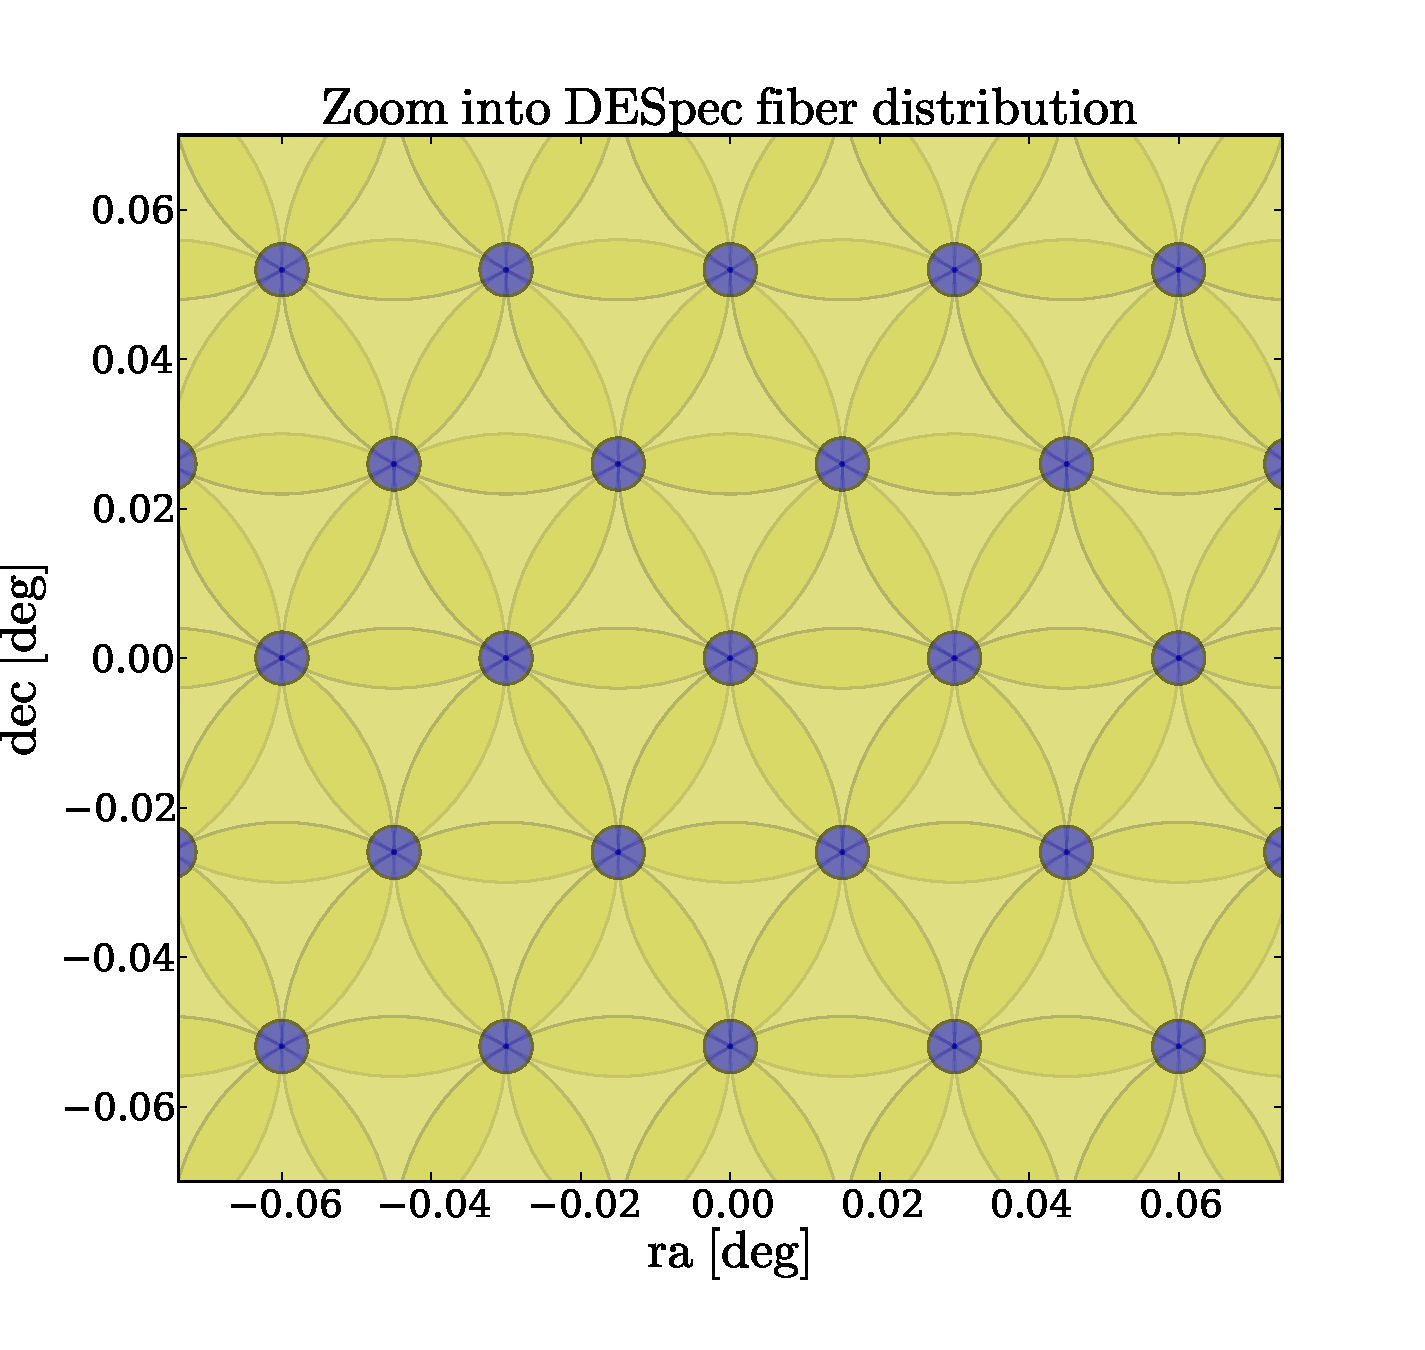
\includegraphics[keepaspectratio=true,width=0.6\textwidth]{DES_fibers_zoom.pdf}
\caption{\label{fig:1}Zoomed in version of the Mohawk fiber
  distribution for the DESpec configuration. Small circles in blue
  indicate the fiber size. Large circles illustrate the patrol
  radius. Regions in light (dark) yellow can be reached by 3 (4)
  fibers.} 
\end{center}
\end{figure}




\begin{figure}
\begin{center}
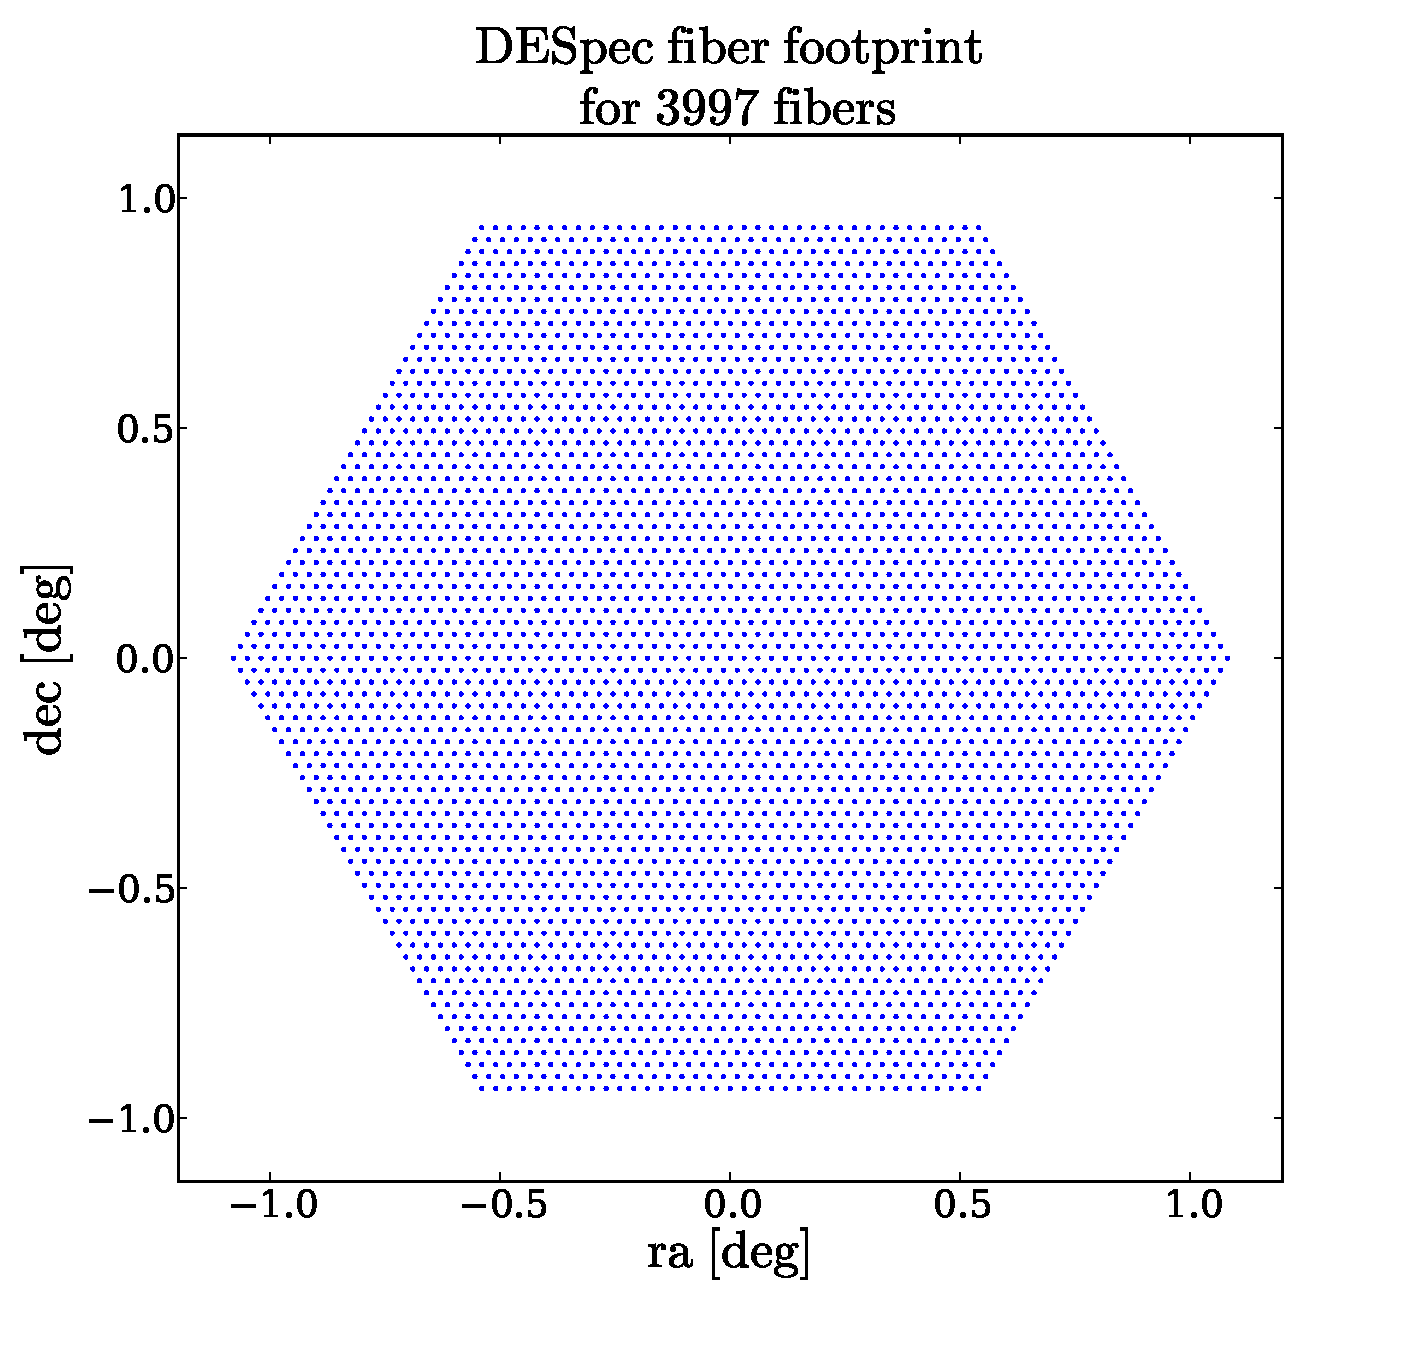
\includegraphics[keepaspectratio=true,width=0.6\textwidth]{DES_fibers.pdf}
\caption{\label{fig:2}Fiber distribution for a DESpec setup.}
\end{center}
\end{figure}


\subsection{Galaxies}



\begin{figure}
\begin{center}
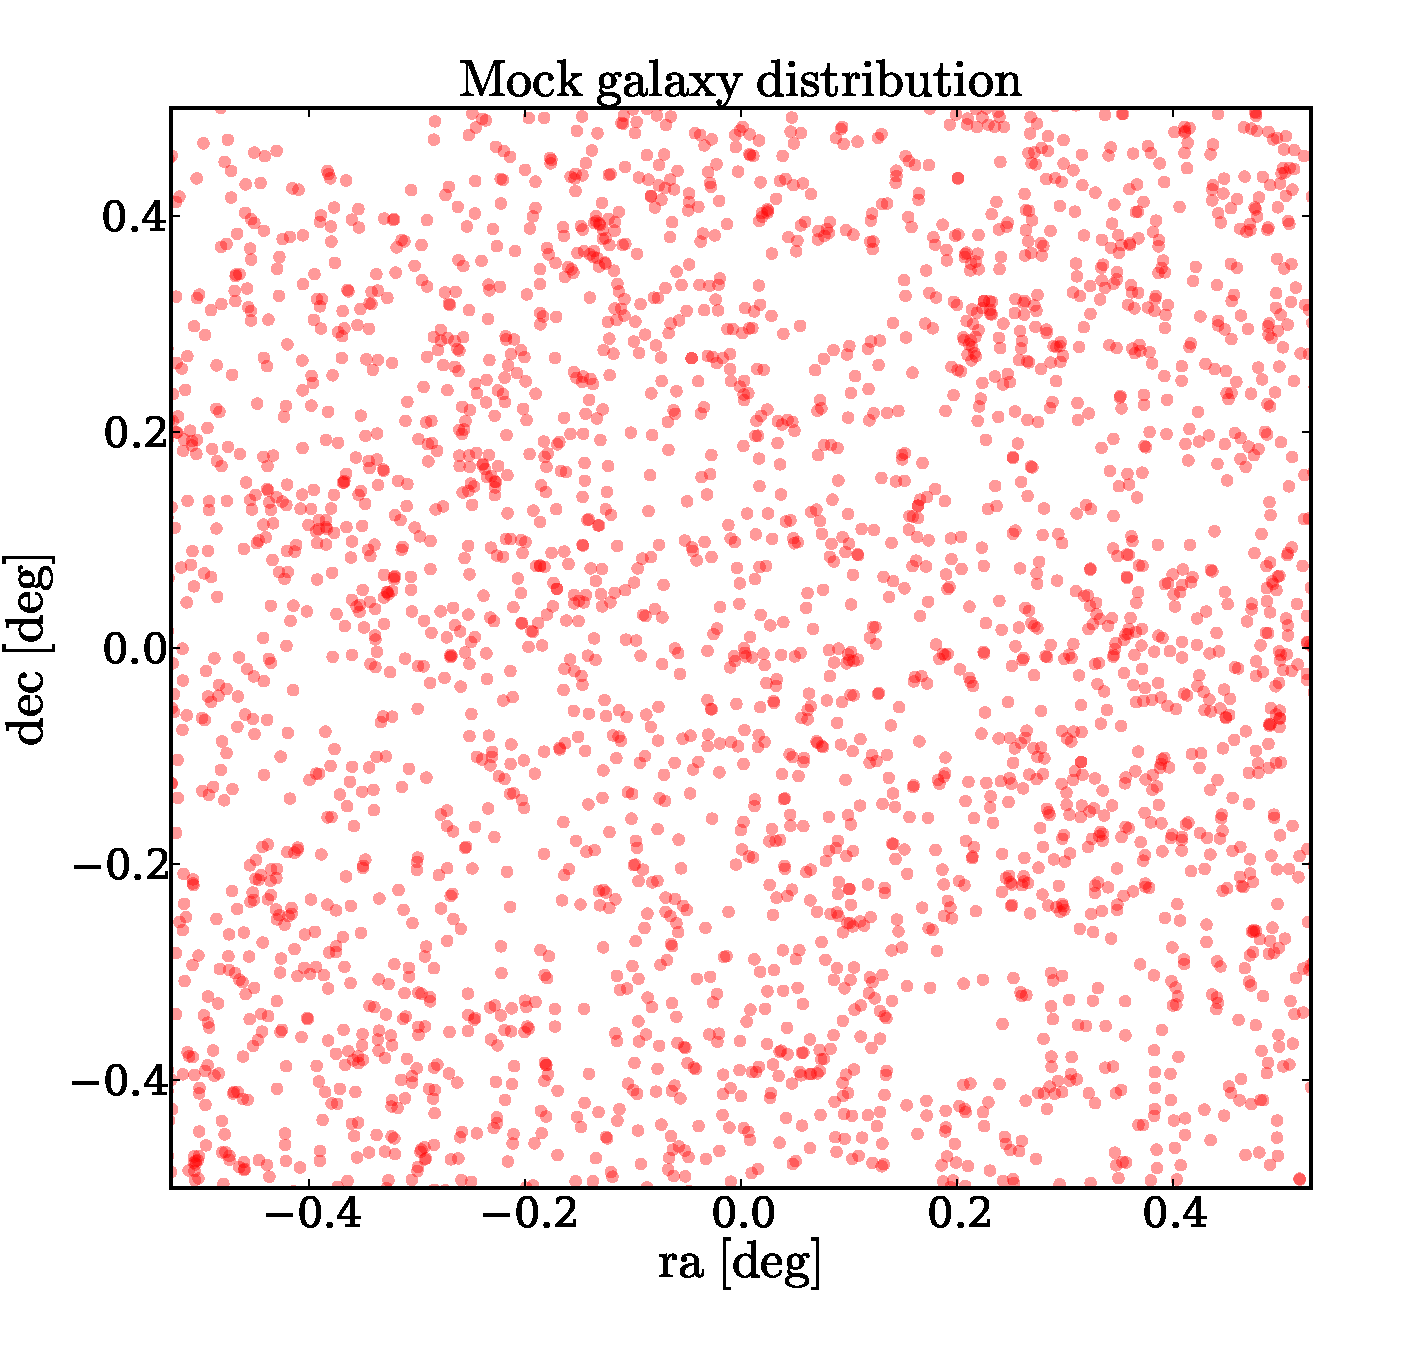
\includegraphics[keepaspectratio=true,width=0.6\textwidth]{mock_gals.pdf}
\caption{\label{fig:3}Mock galaxy distribution. The number density is
  twice the spine number density for the fiducial DESpec setup.} 
\end{center}
\end{figure}

We use two kinds of galaxy distributions: poissonian and clustered. \\ 

The clustered simulations are built directly from the observed COSMOS
catalog of Capak et al. 2008, Ilbert et al. 2009. We refer to this
simulation as the COSMOS Mock Catalog (CMC) (Jouvel et al. 2009). The
COSMOS photometric-redshift catalog (Ilbert et al. 2009) was computed
with 30 bands over 2 deg2 with data from GALEX, Subaru, CFHT, UKIRT,
and Spitzer. It achieves very good photo-z accuracy and low
catastrophic redshift rates. The CMC is restricted to the area fully
covered by HST/ACS imaging, 1.24 deg2 after removal of masked
areas. There are a total of 538,000 simulated galaxies at $i<26.5$,
with a density of roughly 120 gal/arcmin2. AGN, stars, and X-ray
sources were removed from the input COSMOS catalog. Using the best fit
photo-z and template, we first produce simulated magnitudes using DES
filter transmission. 

 We then apply random errors to the simulated magnitudes based on a
 simple magnitude-error relation in each filter. The simulated mix of
 galaxy populations is then, by construction, representative of the
 COSMOS survey as well as the clustering and additional quantities
 measured in COSMOS such as galaxy size, UV luminosity, morphology,
 stellar masses. The CMC is limited to the range of magnitude where
 the COSMOS imaging is complete $i_{AB} \approx 26.2$ for a 5 $\sigma$
 detection (Capak et al. 2007 and 2008). We associate emission-line
 fluxes for each galaxy of the CMC. 

%We model the [OII] emission-line
% using the Kennicutt 1998 calibration for restframe UV-[OII]
 %emission-line flux relation. For the other emission lines, we adopt
 %intrinsic, unextincted flux ratios of [OIII]/[OII] = 0.36; H
 %beta/[OII] = 0.28; H alpha/[OII] = 1.77 and Ly alpha/[OII] = 2
 %(McCall 1985 Moustakas 2006, Kennicutt 2006, Mouhcine 2005, Kennicutt
 %1998). It shows a good agreement with the VVDS observations
% and is valid for the different galaxy population.


We used 2 types of targets: Emission-Line Galaxies(ELG) and Lyman Red
Galaxies (LRG). These galaxy types give the best probability of having
a high spectroscopic success rate. Using the CMC, we use simple
criterion to do the target selection: ELG with
at least 1 line at 5 sigma and a photoz selection to select highest
redshift galaxies. LRGs with $S/N_{\rm continuum}>2$ and a
$photo-z>0.5$.  The final number density in this catalog is twice as
the spine density for Mowhack in the DESpec configuration  ase
described in Section \ref{sec:setups}





\section{Allocation Algorithms}

We use two allocation algorithms

\subsection{Local Galaxy Density}
The first allocation algorithm gives priority is based on the Local
Galaxy Density (LGD). The motivation for this algorithm is give
priority to the galaxies in dense regions.

The first step in the algorithm is estimating for each galaxy the
number of galaxies to be allocated within a patrol radius,
$n_{p}$. Then we calculated for each spine a list of galaxies that can
be reached, this list is ranked in descending order by $n_{p}$. For
each spine the galaxy with the highest $n_{p}$ is allocated. Then the
code checks for fiber collisions, in the case of a collision the two
fibers are reset and the process iterates until the number of fiber
collisions cannot be decreased or the number of collisions is zero. 

The code has been implemented in Python. It takes about 25 seconds to
run on a 3.8GHz processor for a single field of 8000 targets, observed
twice with 4000 spines. Most of the run time is spent in re-setting
the fiber collisions. 


\subsection{Simulated Annealing}
The second allocation algorithm used simulated annealing to find the
optimum configuration. This has been used in allocation algorithms before,
by e.g., \cite{Multi}, and the treatment here broadly follows those
efforts. An allocation is initially made at random. Assignments and
deassignments are then made, also at random, except that deassignments
are slowly made less and less likely to be accepted. This is done by assigning
a 'temperature' T to the system, and accepting deassignments with
probability $\exp(-m_i/T)$, where $m_i$ is the merit of the ith target to be
observed. 1/T was slowly increased, linearly, from 1/(1000 $n_s$ $n_p$) to 10,
where $n_s$ is the number of spines and $n_p$ is the number of passes. $10^4$
$n_pn_s$ trial assignments/deassignments were made in total.

The key to doing these huge numbers of changes in reasonable computation
time is in the efficient tabulation of all the possible spine-target
assignations, and of all the exclusions that prevent any given spine
reassignment. These exclusions may be because (a) the proposed target is
already configured, (b) that it is too close to another configured target,
or (c) that the spine would cross an existing spine-target assignment, when
seen in projection. In actuality, most crossings can be allowed (i.e. the
spines do not physically touch), but the penalty from excluding them is
very small, and allows great simplification of the reconfiguring process
itself. In principle, the algorithm could be more efficient if real
reassignments were allowed, i.e. a spine is switched directly from one
target to another, without deassignment in between. However, this causes a
significant increase in book-keeping complexity and was not pursued at
this stage.

The multiple sets of passes are annealed simultaneously, so the exclusions
can be circumvented by having them on different passes. The home positions
of the spines were kept fixed for the multiple passes, which is not
optimal, especially for the BigBOSS geometry with many passes and highly
asymmetric overlap between patrol areas. 

The annealing source code used to perform the tests presented in this
research note is written in FORTRAN77. The code takes about 80 seconds
to run on a 3.8GHz processor for a single field of 8000 targets,
observed twice with 4000 spines. The run time is about equally divided
between setting up the exclusions and doing the annealing. 




\section{Results}

The following table summarizes our results

\begin{table}[!ht]
\begin{center}
\begin{tabular}{cccccc}\hline
Fiber & Galaxy & Allocation & \% Total & \% ELG & \% LRG\\
Setup & Distribution & Algorithm & Complete. &
Complete.&Complete.\\\hline  
DESpec & Poisson & SA & 95.65 & -& -\\
BB & Poisson & SA & 90.77 & -& -\\
DESpec & Mock & SA & 90.70 & 91.09 & 90.25 \\
BB & Mock & SA & 86.27 & 86.77 & 85.68\\
DESpec & Poisson & LGD & 93.84 & -& -\\
BB & Poisson & LGD & 88.27& -&-\\
DESpec & Mock & LGD & 90.01 & 93.28 & 86.23\\
BB & Mock & LGD & 83.69 & 87.78 & 78.95\\\hline
\end{tabular}
\end{center}
\label{Summary of the results.}
\end{table}



\begin{thebibliography}{10}
\bibitem[Miszalski et al. (2006)]{Multi} Multi-Object Spectroscopy
  Field Configuration by  Simulated Annealing, Brent Miszalski, Keith
  Shortridge, Will  Saunders, Quentin A. Parker, Scott M. Croom,
  MNRAS. 371, 1537-1549  (2006)  
\end{thebibliography}



\end{document}

